\icode{E-MI-SI-L2-261113-001}
如图所示，竖直方向固定一个圆形轨道，其内部恰好对称放置 5 个完全相同、重力均为 $G$ 的光滑均质小球，球 1 和球 5 的重心与轨道圆心 $O$ 在同一高度，5 个小球的重心和圆形轨道的圆心在同一竖直面内，下列说法正确的是\paren[]

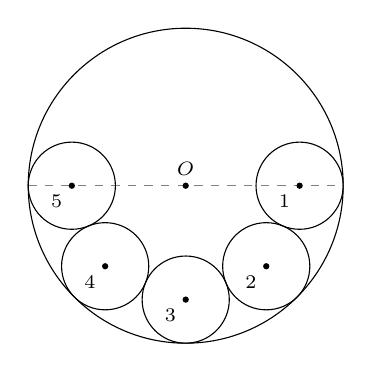
\begin{tikzpicture}[font=\scriptsize]
	\draw[dashed,cyan] (-2,0)--(2,0);
	\fill (0,0)node[above]{\(O\)} circle(.04);
	\foreach \angle/\num in{0/1,-45/2,-90/3,-135/4,-180/5}
		{\draw (\angle:{2-2*sin(22.5)/(1+sin(22.5))}) circle({2*sin(22.5)/(1+sin(22.5))});
		\fill (\angle:{2-2*sin(22.5)/(1+sin(22.5))})node[below left]{\(\num\)} circle(.04);}
	\draw (0,0) circle(2);
\end{tikzpicture}
\begin{choices}
	\item 轨道对球 1、球 5 的作用力相同
	\item 球 2 和球 4 对球 3 作用力的合力方向竖直向下
	\item 球 2 对球 1 的作用力大小可能小于 $G$
	\item 轨道对球 3 的作用力大小等于 $5G$
\end{choices}
\begin{answer}
	B\qquad 提示：
\end{answer}